%http://cs.pugetsound.edu/~jross/courses/cs240/project/requirements/
%Animation Group
\documentclass[12pt]{article}
\usepackage{graphicx}
\begin{document}

% Front Page
\begin{titlepage}
	\begin{center}
	\huge  Edith \\
	\vspace*{\fill}%
 	\huge \textsc{\textbf{Animation System \\Intermediate Report} }	
	\bigskip 
	\rule{130mm}{.1pt}
	\textsc{\textbf{October 7, 2013 \\ Revised: October 17, 2013} \\ }	
	\vspace*{\fill}%
	Eric Lund \\
	Kramer Canfield \\ 
	Zeke Rosenberg \\
	Calder Whiteley \\
	Jon Youmans
	\end{center}
\end{titlepage}

\section{\emph{Animation System Structure}}%Create a section for the introduction
\begin{enumerate}
\item Parser
\begin{enumerate}
\item The Animation System will be receiving instructions for animations in JSON format. This subsystem will take the instructions and actually call the functions with correct inputs. Our required interface is JSON, but more specifically a JSON entry with the following elements:
\item \{``function name" : ``jump(x1, x2, y1, y2)", ``Image Name": ``example.png", ``Audio File Name": ``soundFile.mp3"\}
\item There will be certain instructions that might not have specific pieces of information, such as an animation without an associated sound. In a case where this occurs, input ``null" in the appropriate location.
\end{enumerate}

\item Controller
\begin{enumerate}
\item Once we have parsed JSON inputs into separate instructions, the Controller subsystem will carry out those instructions and send media creation and display instructions to the HTML5 canvas. This component will have several important interactions.
\item The Controller will take the raw data about the media instructions and creates a list of instructions to send to the HTML5 canvas. The instructions for the canvas will be stored in a Scene Array, which will later be useful for play(), pause(), and seek().
\end{enumerate}

\item Scene Array
\begin{enumerate}
\item The Scene Array sub-component simply holds a list of frames, each frame being one step of the animation process. These will be stored in an array so that playback control functions (called by another team) will allow the user to select a time to view from, and the Scene Array can then get the necessary media and display it. 
\end{enumerate}

\item Interactions
\begin{enumerate}
\item The Animation System will have no direct interaction with the ``programmer" because the Animation System is a back-end module and is dependent on other frameworks and modules such as a canvas.
\item The Animation System interacts with the Story Creator module, who feeds us the JSON instructions to be interpreted with the parser and carried out. It also interacts with the visual editor team, which will be providing the images, sounds, etc. to be used following the JSON instructions. Finally, we will be giving our output to the (some other team here) to be painted on the canvas.
\item The only other requirement for the Animation System is that we are using a 3rd party library, ``OCanvas', to make animations easier and better looking. This library works directly with an HTML5 canvas, so there are minimal if any changes from other teams. This can be found at http://ocanvas.org/docs

\end{enumerate}



\end{enumerate}

\subsection{Activity Diagram}
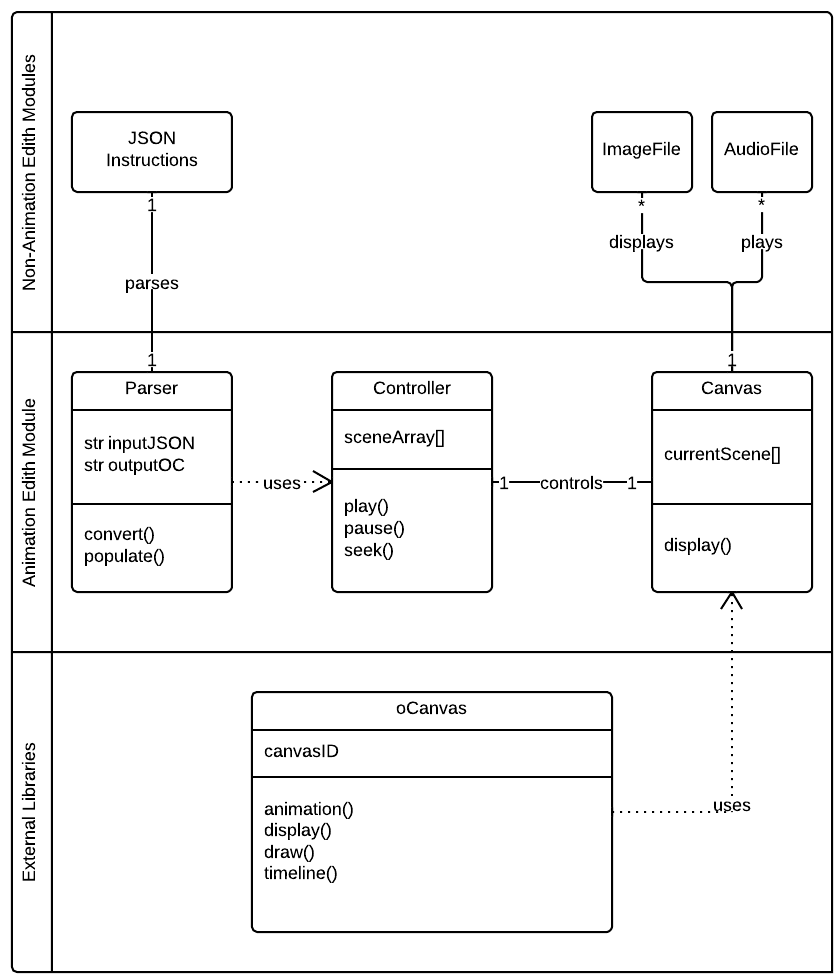
\includegraphics[scale=.45]{AnimationUMLClassDiagram.png}
\\UML Class Diagram
\pagebreak

%Glossary/References
\section{\emph{Glossary/References}}
Glossary:
\begin{itemize}
	\item Programmer: The individual who is using Edith through his/her web browser to learn how to program.
	\item Sprite: a computer graphic that may be moved on-screen and otherwise manipulated as a single entity (New Oxford American Dictionary (American English))
\end{itemize}
	

	
\end{document}
